\documentclass{standalone}
\usepackage{pgfplots}
\pgfplotsset{compat=newest}

\begin{document}
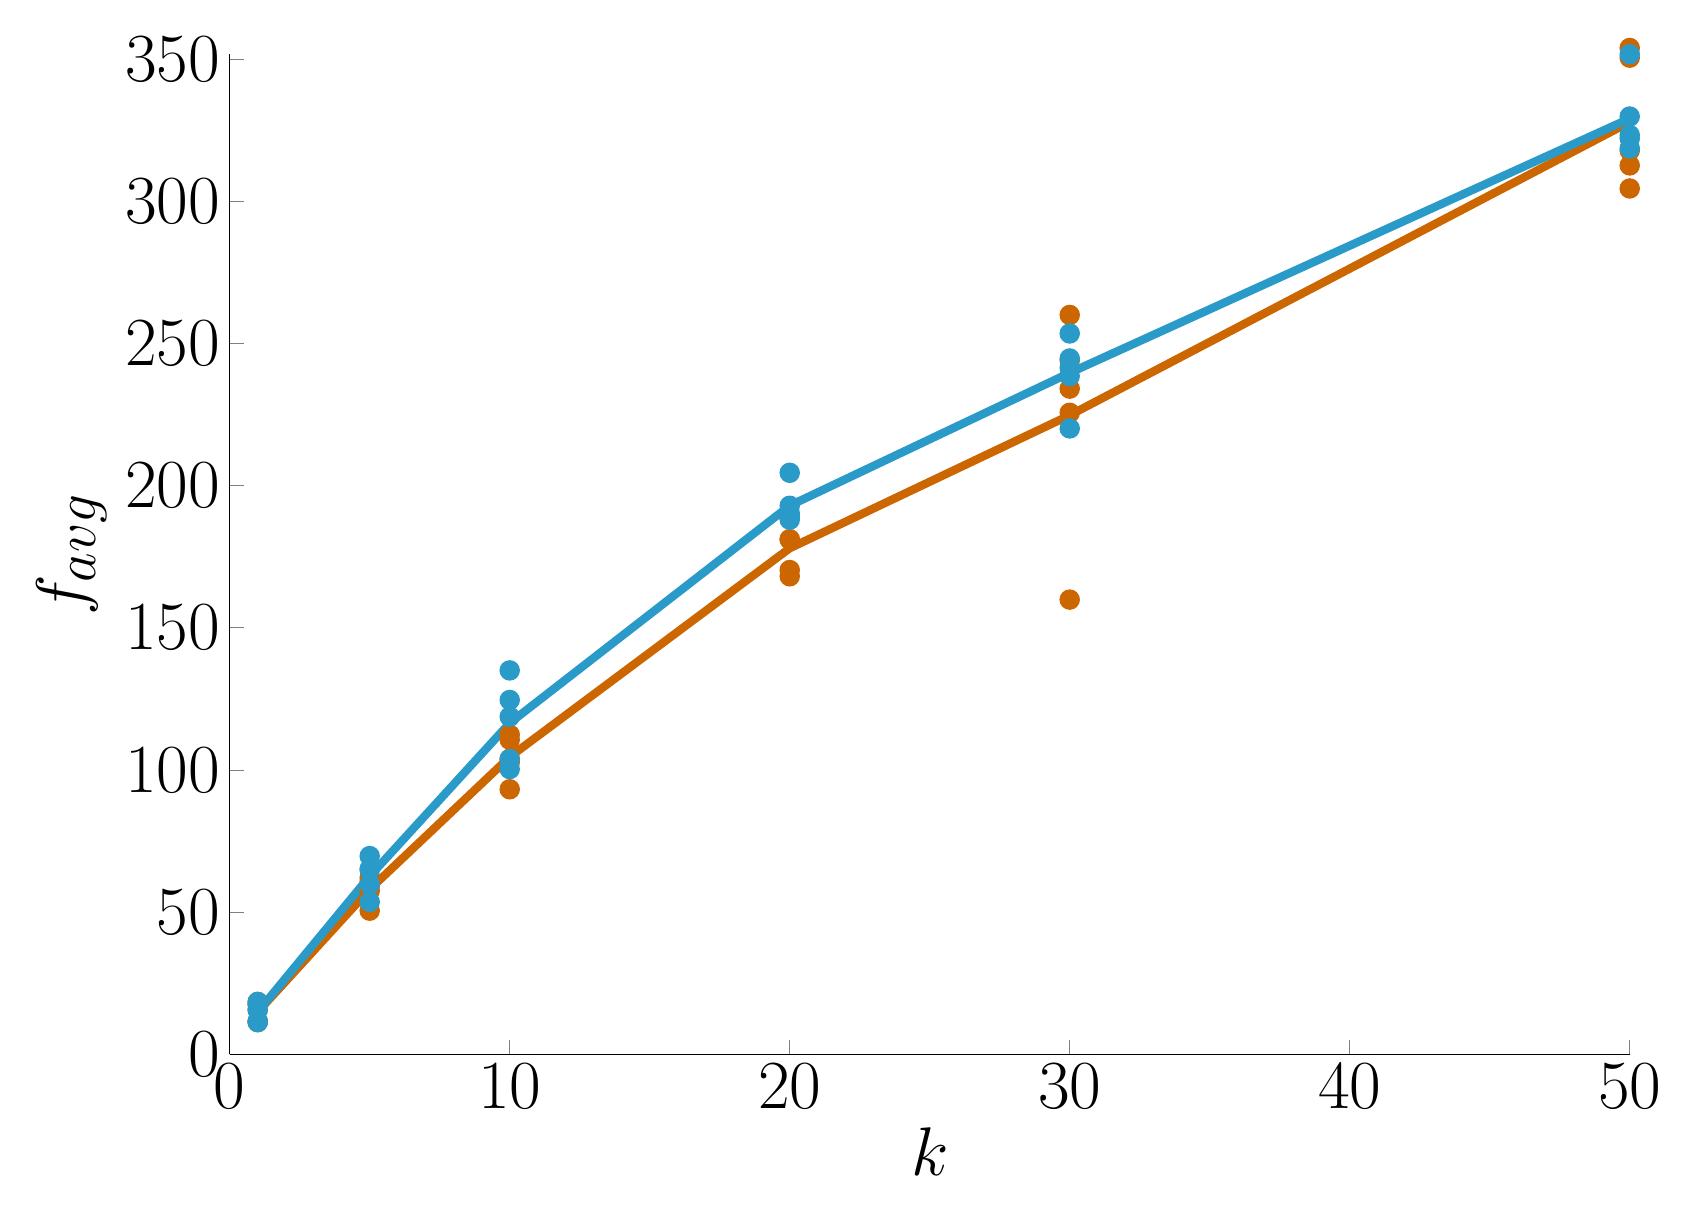
\begin{tikzpicture}

\begin{axis}[%
tick label style={font=\Huge},
label style={font=\Huge},
legend style={font=\Huge},
view={0}{90},
max space between ticks=50pt,
width=7in,
height=5in,
scale only axis,
xmin=0, xmax=50,
xtick={0, 10, 20, 30, 40, 50},
xlabel={$k$},
ymin=0, ymax=351.7,
%ytick={0, 200, 400, 600, 800, 1000},
ylabel={$f_{avg}$},
major tick length=5pt,
axis lines*=left,
legend cell align=left,
clip=false]

\addplot [
only marks,
mark=*,
mark size=3.5pt,
color=orange!80!black,
%solid,
%line width=2pt,
]
coordinates{
(1,11.3)(1,11.6)(1,15.6)(1,17.5)(1,18.4)(5,50.5)(5,57.5)(5,59.1)(5,60.8)(5,62.1)(10,93.2)(10,102.7)(10,103.9)(10,110.6)(10,112.4)(20,168.1)(20,170.3)(20,181.1)(20,181.1)(20,189.2)(30,159.9)(30,225.6)(30,234.1)(30,244.1)(30,260.0)(50,304.5)(50,312.6)(50,317.8)(50,350.5)(50,353.9)
};

\addplot [
only marks,
mark=*,
mark size=3.5pt,
color=cyan!80!black,
%solid,
%line width=2pt,
]
coordinates{
(1,11.3)(1,11.6)(1,15.6)(1,17.5)(1,18.4)(5,53.6)(5,59.8)(5,64.8)(5,65.2)(5,69.7)(10,100.3)(10,103.8)(10,118.7)(10,124.6)(10,135.0)(20,188.0)(20,189.0)(20,190.3)(20,192.9)(20,204.5)(30,220.1)(30,238.5)(30,241.4)(30,244.7)(30,253.5)(50,318.6)(50,322.1)(50,323.3)(50,329.8)(50,351.7)
};

\addplot [
color=orange!80!black,
solid,
line width=3pt
]
coordinates{
(1,14.88)(5,58.0)(10,104.56)(20,177.96)(30,224.74)(50,327.86)
};

\addplot [
color=cyan!80!black,
solid,
line width=3pt
]
coordinates{
(1,14.88)(5,62.62)(10,116.48)(20,192.94)(30,239.64)(50,329.1)
};


\end{axis}
\end{tikzpicture}
\end{document}
